\section{Overhead}

One of our first concerns was to implement a framework that does not impact our simple application.
The benchmarking framework should be hidden for the developer.
Enabling the framework should not alter the good use of the application.

To measure the impact of our approaches, we used the same setup as with our reference value and retrieved 1000 measurements of the context switching time.
We compared those measurements with our reference value and computed the overhead of our framework.
The oscilloscope measurements are shown in the figure \ref{fig:overhead-reference-value-contiki-z1}.

\subsection{Extension approach overhead}

The extension approach has a large overhead of more than 2 ms for with RE-Mote board and more than 3 ms with the Z1 board on both Contiki and RIOT.
In the figure \ref{fig:overhead-extension-contiki-z1}, we can see the overhead of the first approach with the measurements made with the oscilloscope.
We discuss later why our extension approach adds so much latency in the section \ref{sec:overhead}.

\subsection{Devices approach overhead}

The devices approach, on the other hand, has a small overhead of less than 3 $\mu$s with either the RE-Mote or the Z1 boards on both Contiki and RIOT.
In the figure \ref{fig:overhead-devices-contiki-z1}, we can see the overhead of the devices approach.
The devices approach adds a much smaller overhead to our simple application than the extension approach.
This difference between the overhead of the two approaches is discussed in the section \ref{sec:overhead}.

\begin{figure}[!ht]
        \centering
        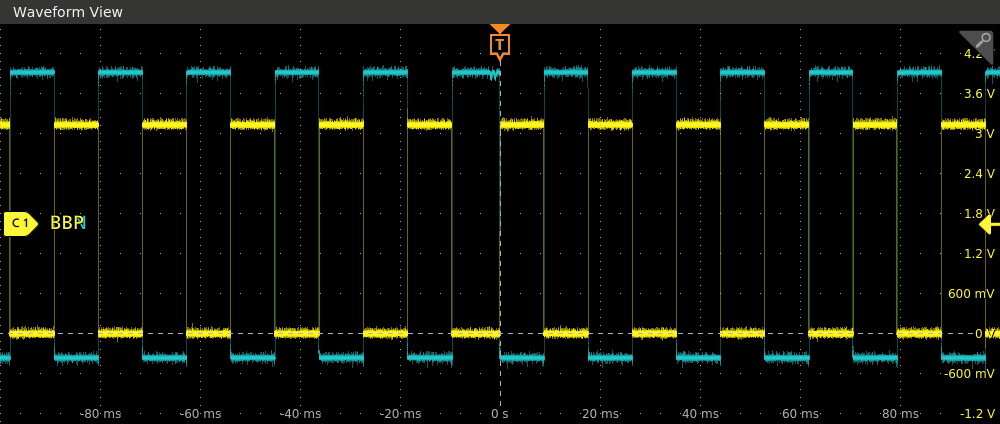
\includegraphics[scale=.4]{assets/reference-value-overhead-contiki-z1.png}
        \caption{overhead reference measured by the oscilloscope\label{fig:overhead-reference-value-contiki-z1}}

        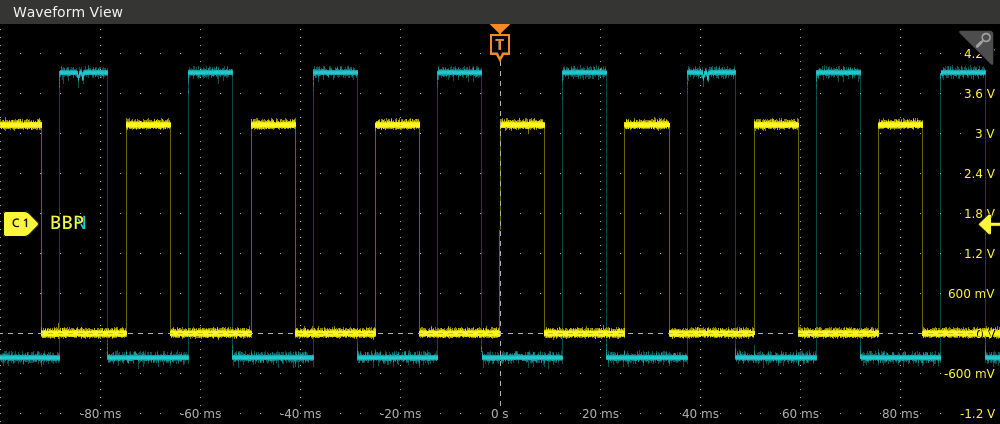
\includegraphics[scale=.4]{assets/extension-framework-overhead-contiki-z1.png}
        \caption{extension approach overhead measured by the oscilloscope\label{fig:overhead-extension-contiki-z1}}

        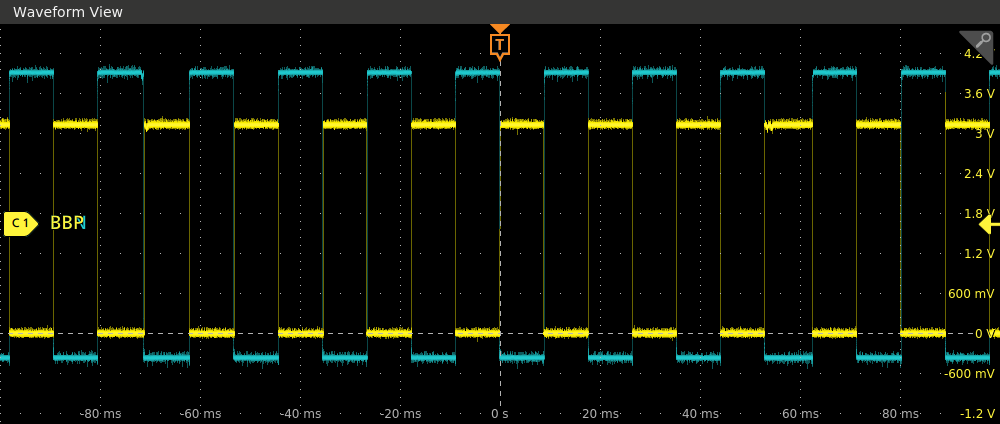
\includegraphics[scale=.4]{assets/devices-framework-overhead-contiki-z1.png}
        \caption{devices approach overhead measured by the oscilloscope\label{fig:overhead-devices-contiki-z1}}
\end{figure}